%-------------------------------------
%            Disclaimer
 %This is a template developed from:
 %https://www.overleaf.com/latex/templates/imperial-college-individual-project-template/bhgyjxmsvwqj
 % comes from License Creative Commons CC BY 4.0
 % The template at ESPOCH should be used for academic or research purpose. For any additional detail follow the link shared above.

 % Modified by xavysp with the aim of academic usage at Escuela Superior Politécnica de Chimborazo (ESPOCh)---Polytechnic School of Chimborazo in English at Morona-Santiago Ecuador. 
% ----------------------------------

\documentclass[12pt,a4paper, twoside]{report}
\setcounter{secnumdepth}{4}
\usepackage{sectsty}
\allsectionsfont{\normalsize}
%% Language and font encodings
\usepackage[english, spanish]{babel}
\usepackage[utf8]{inputenc}
\usepackage[T1]{fontenc}

%% Sets page size and margins
\usepackage[a4paper,top=3cm,bottom=2cm,left=3cm,right=3cm,marginparwidth=2cm]{geometry}

%% Useful packages
% \usepackage[backend=biber,style=imperialharvard]{biblatex}
\usepackage[backend=biber,style=iso-authoryear]{biblatex}

% \usepackage[backend=biber,style=iso-authoryear]{biblatex}
% style=iso-authoryear,iso-numeric,iso-alphabetic,iso-authortitle
% mayor información sobre citas con norma ISO 690: https://biblioteca.uoc.edu/en/page/ISO-690-style/

% En castellano: https://biblioguias.uam.es/citar/estilo_une


\usepackage{afterpage}
\usepackage{amsmath}
\usepackage{amsthm}
\usepackage{csquotes}
\usepackage{enumitem}
\usepackage{graphicx}
\usepackage{lipsum}
\usepackage{booktabs}
\usepackage{float}
\usepackage[figuresright]{rotating}% rotate pages
% \usepackage{typearea} % help to change the page horientation

% Listings (for displaying code):
\usepackage{listings}
\lstset{
    frame = single, 
    framexleftmargin=15pt
}

% Center figure captions:
\usepackage[labelfont=bf,justification=centering]{caption}

% ----------- Algorithm2e setup
\usepackage[ruled,vlined]{algorithm2e}
\makeatletter
\renewcommand{\SetKwInOut}[2]{%
  \sbox\algocf@inoutbox{\KwSty{#2}\algocf@typo:}%
  \expandafter\ifx\csname InOutSizeDefined\endcsname\relax% if first time used
    \newcommand\InOutSizeDefined{}\setlength{\inoutsize}{\wd\algocf@inoutbox}%
    \sbox\algocf@inoutbox{\parbox[t]{\inoutsize}{\KwSty{#2}\algocf@typo:\hfill}~}\setlength{\inoutindent}{\wd\algocf@inoutbox}%
  \else% else keep the larger dimension
    \ifdim\wd\algocf@inoutbox>\inoutsize%
    \setlength{\inoutsize}{\wd\algocf@inoutbox}%
    \sbox\algocf@inoutbox{\parbox[t]{\inoutsize}{\KwSty{#2}\algocf@typo:\hfill}~}\setlength{\inoutindent}{\wd\algocf@inoutbox}%
    \fi%
  \fi% the dimension of the box is now defined.
  \algocf@newcommand{#1}[1]{%
    \ifthenelse{\boolean{algocf@inoutnumbered}}{\relax}{\everypar={\relax}}%
%     {\let\\\algocf@newinout\hangindent=\wd\algocf@inoutbox\hangafter=1\parbox[t]{\inoutsize}{\KwSty{#2}\algocf@typo\hfill:}~##1\par}%
    {\let\\\algocf@newinout\hangindent=\inoutindent\hangafter=1\parbox[t]{\inoutsize}{\KwSty{#2}\algocf@typo:\hfill}~##1\par}%
    \algocf@linesnumbered% reset the numbering of the lines
  }}%
\makeatother
% --------- end algorithm2e setup

% \bm allows typing bold math:
\usepackage{bm}

% -------- Fancy page headers:
\usepackage{fancyhdr}
\pagestyle{fancy}
\fancyhf{}
\fancyhead{}
%RO,LE \MakeUppercase
\fancyhead[RO,LE]{\MakeUppercase{\leftmark\hfill}}
\fancyfoot[LE,RO]{\hfill\thepage\hfill}
\setlength{\headheight}{15.6pt}

% -------- Finish setting up fancy page headers


% ---------- Setup for definitions:
\usepackage{tipa}
\usepackage{tcolorbox}
\usepackage{xcolor}
\definecolor{mdgrey}{rgb}{0.8, 0.8, 0.8}
\usepackage[framemethod=tikz]{mdframed}
\usepackage{lipsum}
\newtheoremstyle{defi}
  {\topsep}%
  {\topsep}%
  {\normalfont}%
  {}%
  {\bfseries}% 
  {:}%
  {.5em}%
  {\thmname{#1}\thmnote{~(#3)}}%
\theoremstyle{defi}
\newmdtheoremenv{definitioni}{Definition}
\newmdtheoremenv[
hidealllines=true,
leftline=true,
innertopmargin=0pt,
innerbottommargin=0pt,
linewidth=4pt,
linecolor=gray!40,
innerrightmargin=0pt,
]{definitionii}{Definition}
\newmdtheoremenv[
roundcorner=5pt,
innertopmargin=0pt,
innerbottommargin=5pt,
linewidth=4pt,
linecolor=gray!40,
]{definitioniii}{Definition}
% ---------- End setup for definitions

\usepackage[colorinlistoftodos]{todonotes}
\usepackage[colorlinks=true, allcolors=gray]{hyperref}

\renewcommand*{\rmdefault}{bch}
\renewcommand*{\ttdefault}{lmtt}
\newcommand{\citationneeded}{\textcolor{red}{[citation-needed]}}

\addto\captionsenglish{% Replace "english" with the language you use
  \renewcommand{\contentsname}%
    {ÍNDICE GENERAL}% the custom name of table of contents
  \renewcommand{\listfigurename}{LISTA DE FIGURAS}
    \renewcommand{\listtablename}{LISTA DE TABLAS}
    \renewcommand{\figurename}{Figura}
    \renewcommand{\chaptername}{CAPÍTULO}
}
\renewcommand{\tablename}{Tabla}
\renewcommand{\algorithmcfname}{Algoritmo}


% Set chapter title
\usepackage{titlesec, titletoc}

\titleformat{\chapter}[display]
  {\large \bfseries \centering}{\MakeUppercase{}}{0pt}{\large\MakeUppercase}
\titlespacing*{\chapter}{-10pt}{-20pt}{25pt}

\titlecontents{chapter}[0.2em]{\bigskip\bfseries}%\vspace{1cm}%
{\contentslabel[\MakeUppercase{}]{7em}\MakeUppercase}%
{\MakeUppercase}%numberless chapters%
{\hfill\contentspage}[\medskip]%
% End set chapter title
% -------------------------
% --------------------------

\DeclareMathOperator*{\argmin}{\arg\!\min}
\DeclareMathOperator*{\argmax}{\arg\!\max}

\title{Aquí el título de la propuesta}

% Uncomment if you want a subtitle:
% \vspace{1em}\large Interim Report}

\author{Nombres y apellidos}
% Update supervisor and other title stuff in title/title.tex

% Add bigger skip between paragraphs, makes reading easier:
\setlength{\parskip}{0.5em}

\bibliography{bibs/bibliography.bib}

\begin{document}
\begin{titlepage}

\newcommand{\HRule}{\rule{\linewidth}{0.5mm}} % Defines a new command for the horizontal lines, change thickness here

%----------------------------------------------------------------------------------------


\center % Center everything on the page
\textsc{\LARGE \textbf{Escuela Superior Politécnica de Chimborazo}}\\[0.2cm] %[1.5cm] % Name of your university/college
\textsc{\Large Sede Morona Santiago}\\[1.5cm] % 
%----------------------------------------------------------------------------------------
%	LOGO SECTION
%----------------------------------------------------------------------------------------


\includegraphics[width=10cm]{title/espochTI.png}\\[1.5cm] % Include a department/university logo - this will require the graphicx package
 
%----------------------------------------------------------------------------------------

%	HEADING SECTIONS
%----------------------------------------------------------------------------------------
% Major heading such as course name
\textsc{\large PROPUESTA DE
TRABAJO DE INTEGRACIÓN CURRICULAR}\\[0.5cm] % Minor heading such as course title

%----------------------------------------------------------------------------------------
%	TITLE SECTION
%----------------------------------------------------------------------------------------
\makeatletter
{\color{red}\HRule} \\[0.6cm]
{ \huge\bfseries \@title}\\[0.6cm] % Title of your document
{\color{red}\HRule}\\[1.5cm]
 
%----------------------------------------------------------------------------------------
%	AUTHOR SECTION
%----------------------------------------------------------------------------------------

\begin{minipage}{0.4\textwidth}
\begin{flushleft} \large
\emph{Autor (es):}\\
Autor 1\\ %\@author % Your name\\
Autor 2
\end{flushleft}
\end{minipage}
~
\begin{minipage}{0.4\textwidth}
\begin{flushright} \large
\emph{Director(a) propuesto:} \\
Mgtr./Dr. Nombres y apellidos aquí \\[1.2em] % Supervisor's Name
% Magister Mgtr, Master Mtr.
% Master o Magister en Ciencias M.Sc. MSc
% Doctor (Cuarto nivel) Dr. / Ph.D. / PhD.

\end{flushright}
\end{minipage}\\[2cm]
\makeatother

% If you don't want a supervisor, uncomment the two lines below and remove the section above
% \Large\@author\\[3cm] % Your name

%----------------------------------------------------------------------------------------
%	DATE SECTION
%----------------------------------------------------------------------------------------
\emph{\large \textbf{Tipo de Trabajo de Integración Curricular:}} \\[0.25cm]
Proyecto de Investigación: [x]\\
Proyecto Técnico: [ ]\\
Emprendimiento: [ ]\\[0.5cm]

{\large Fecha de presentación :}\\[0.1cm]
{\large \today}\\[2cm] % Date, si necesita poner otra fecha elimine \today

\vfill % Fill the rest of the page with whitespace

\end{titlepage}

% \begin{abstract}
% Your abstract goes here
% \end{abstract}
% 
% \renewcommand{\abstractname}{Acknowledgements}
% \begin{abstract}
% Thanks mum!
% \end{abstract}
\pagenumbering{arabic} % starting the page numbering
\tableofcontents

% Inputs:
% Uncomment or add folders to add your own chapters and input files.
% agregamos los capítulos

\chapter{DATOS GENERALES}

\section{Información de la propuesta}
% Poner título de la propuesta
kfncbvmncxbvmxncbvmxcnvbxcxcmvnx

\section{Línea de investigación}
% Poner línea y programas de investigación

\section{Proponentes}
% Autores
\noindent Kaento Vidal Juank Huachapá.

\section{Propuesta de los miembros del tribunal}

\subsection{Director}

\subsection{Tribunal}
% El tribunal para la defensa es designado por CUIC y deben ponerlo solo en la versión final de la propuesta.

\section{Lugar e institución donde se realizará el trabajo de titulación}

%% ---------------------
% A apartir de aquí elimine todo lo que quiera
%% -----------------------

% \begin{definitionii}
% \textbf{\emph{dissertation}}
% \textipa{[dis@\super rteiS\super @n]}
% dɪsəʳteɪʃən

% \noindent   
% A dissertation is a long formal piece of writing on a particular subject, especially for a university degree.

% \noindent \emph{He is currently writing a dissertation on the Somali civil war.}

% \hfill -- Collins English Dictionary \autocite{Smith1998}
% \end{definitionii}

Above you will find a nicely typeset definition.

\begin{figure}
    \centering
    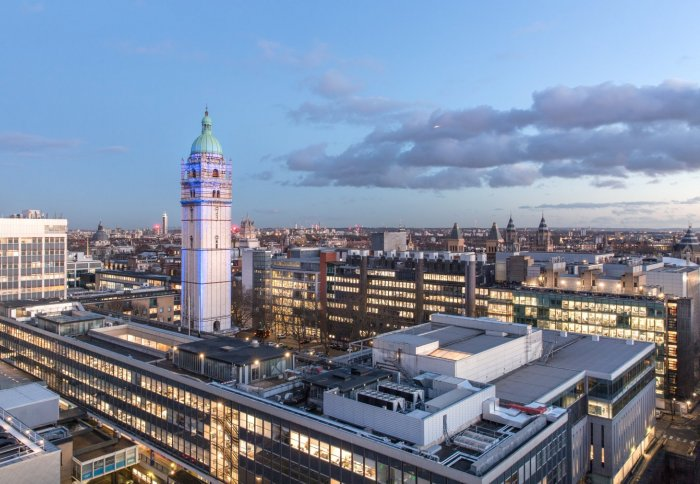
\includegraphics[width=5cm]{img/imperial.jpg}
    \caption{Una prueba}
    \label{fig:intro}
\end{figure}

Como se muestra en la figura \ref{fig:intro}, nuestro problema....

\begin{table}
    \centering
    \begin{tabular}{llr}  
        \toprule
        \multicolumn{2}{c}{Item} \\
        \cmidrule(r){1-2}
        Animal    & Description & Price (\$) \\
        \midrule
        Gnat      & per gram    & 13.65      \\
                  &    each     & 0.01       \\
        Gnu       & stuffed     & 92.50      \\
        Emu       & stuffed     & 33.33      \\
        Armadillo & frozen      & 8.99       \\
        \bottomrule
    \end{tabular}
    \caption{Example booktabs table \cite{ramzan2019noSQLsecure}. Booktabs tables are nicer than regular ones, in my opinion. This site has a nice GUI for making LaTeX tables, and has a Booktabs option: https://www.tablesgenerator.com/}
    \label{tab:my_label}
\end{table}

\lipsum[1-4] Table \ref{tab:my_label}

\section{Section Example}
\lipsum[1]
\subsection{Subsection Example}
\label{subsection:example}
\lipsum[1]
\subsubsection{Subsubsection Example}

Note that you can reference chapters, sections, subsections and subsubsections. For example: Subsection \ref{subsection:example}

\section{Math Example}

\begin{equation}
\textrm{score}(x) = \left(\lambda_m\sum_{i=0}^{|\mathbf{m}|} \log \hat{p}_m(d(x, \mathbf{m}_i) \mid l_i)\right) + \left(\lambda_l\sum_{i=0}^{|\mathbf{l}|} \log\hat{p}_l(d(x, \mathbf{l}_i) \mid \mathbf{v}_i)\right) + \lambda_p \hat{p}_p(x)
\end{equation}

\section{Algorithm Example}

See Algorithm \ref{algorithm:posit}

\begin{algorithm}
\SetAlgoLined
\SetKwInOut{KwInput}{Input}
\SetKwInOut{KwOutput}{Output}
\SetKwInOut{KwPre}{Pre}
\SetKw{Return}{return}
\SetKwProg{Fn}{Function}{}{end}
\LinesNumbered
\KwInput{$\textbf{m}$, such that $\mathbf{m}_i$ is the position of the $i$'th monitor\newline
$\textbf{l}$, such that $\mathbf{l}_i$ is the position of the $i$'th landmark\newline
$\mathbf{p}^m$, such that $\mathbf{p}^m_i$ is the ping latency from monitor $i$ to the target\newline
$\mathbf{p}^l$, such that $\mathbf{p}^l_i$ is the set of ping latencies to landmark $i$}

\BlankLine
\KwPre{Compute $\hat{p}_m(d \mid l)$, an estimator giving the likelihood of the target being distance $d$ away from the monitor, given that the monitor records a latency of $l$ to that target. Implemented by training a KDE using $\mathbf{p}^l$.\newline
Compute $\hat{p}_l(d \mid v)$, an estimator giving the likelihood of the target being distance $d$ away from the landmark, given a Canberra distance of $v$ between the target and the landmark, using training targets.
}
\BlankLine
\KwOutput{Most likely location of the target}
\BlankLine

\Fn{Likelihood($x$, $\mathbf{v}$)} {
MonitorScore $\gets \sum_{i=0}^{|\mathbf{m}|} \log{\hat{p}_m(d(x, \mathbf{m}_i) \mid l_i)}$\;
LandmarkScore $\gets \sum_{i=0}^{|\mathbf{l}|} \log{\hat{p}_l(d(x, \mathbf{l}_i) \mid \mathbf{v}_i)}$\;
\Return MonitorScore + LandmarkScore
}

\BlankLine
$\mathbf{v} \gets $\{$\mathrm{canberra\_distance}(\mathbf{l}_i, \mathbf{p}^m) \mid \mathbf{l}_i \in \mathbf{l}$\}

$\mathbf{C}$ $\gets$ Constraint-Based-Geolocation($\mathbf{m}$, $\mathbf{p}^m$)\;
$\mathbf{C_l}$ $\gets$ \{$m \in \mathbf{m} \mid \mathbf{C}$ contains $m\} \cup \{l \in \mathbf{l} \mid \mathbf{C}$ contains $l$\}\;
\BlankLine
\Return argmax$_{x\in \mathbf{C_l}}$ Likelihood($x$)

 \caption{Algorithm example}
 \label{algorithm:posit}
\end{algorithm}

%% ----------------------
% Puede eliminar hasta aquí
%% ----------------------
\chapter{Formulación del trabajo de integración curricular} % poner en mayus

\section{Problema}


\subsection{Antecedentes}
% Detallar investigaciones relacionadas o similares. Por ejemplo si una persona desarrollo una aplicación de citas ponerlo indicando los logros alcanzados, el objetivo con el que se creó y las conclusiones a las que llegó. Revisar estado del arte.
Aquí ponemos cómo hacer \textbf{citas narrativas}... como menciona \textcite{yaqoob2016BDfuture} "la vida es bella", disfruta.

Aquí ponemos cómo hacer \textbf{citas parentéticas}. En la vida nos podemos encontrar con tropiezos pero más allá de eso la vida es bella \parencite{yaqoob2016BDfuture}.
 


\subsection{Formulación del problema}
% Decribir el problema actual
% 

\section{Justificación de la propuesta}
% contrar cómo la propuesta ayudará a resolver este problema

\subsection{Justificación teórica}


\subsection{Justificación aplicativa}

\section{Objetivos}

\subsection{Objetivo general}
\subsection{Objetivos específicos}

\section{Hipótesis y preguntas de investigación} % La hipótesis solo se definirá para proyectos de investigación que involucren operacionalizar variables e indicadores. 


\section{Marco teórico} % 2-4 páginas

\subsection{Conceptos y generalidades}



\subsection{Estado del arte} %Es el alcance de la investigacón hasta la fecha. Es decir, si usted propone el desarrollo de una aplicación de citas, bascar investigaciones actuales  relacionados a su tema, Aquí debe poner, los tipos de algorítmos utilizados para hacer el match (emparejamiento) el diseño del software, pruebas de implementación.

% podríamos poner lo de temario tentativo desglosado




\chapter{Metodología de la investigación} % para Proyecto de investigación
% \chapter{Metodología de desarrollo} % para Proyecto técnico

\section{Metodología}
% Si el trabajo a realizar son propuestas técnicas,  la metodología a emplear será afín al tema planteado y los puntos abajo citados deberán desarrollarse en base al producto final a oftener.
% Aquí debe decribir la metodología de la propuesta

\subsection{Enfoque} % para Proyecto de investigación
% cuantitativa, cualitativa o mixta

\subsection{Alcance} % tamaño del proyecto
% explicar la profundidad o hasta donde llegará el proyecto de investigación o técnico

\subsection{Tipos} % para proyecto de investigación
% Exploratoria, descriptiva, explicativa, etc.

\subsection{Métodos} % para proyecto de investigación
% inductivo, deductivo, etc.% 

\subsection{Diseño}


% Para proyecto de investigación: experimental, correlacional, cuasi-experimental, etc.
% Para proyecto técnico: descripción de escenarios o ambientes de pruebas.



\subsection{Sistematización de la investigación}
% En el caso de proyectos de investigación  operacionalizar variables de investigación a partir de una hipótesis.
% En el caso de proyecto técnicos se debe indicar los parámetros de evaluación del producto final. Los mismo deben estar basados en estándares de calidad o extraido de la literatura.

% Fin metodologias de investigación

\section{Técnicas e instrumentos de investigación} % Para proyecto de investigación:

% Detallar el tratamiento de los datos y su recolección

\section{Recursos}
% preparar una introducción breve del tiempo de duración de la propuesta
\subsection{Hardware}





\subsection{Software}
%  Hardware, software, humanos
\subsection{Presupuesto}
Como se puede observar en la Tabla \ref{tab:presu}.
\newpage
% para trabajar con imagen en vez de table puedes usar
% \begin{sidewaysfigure} ... \end{sidewaysfigure}

\begin{sidewaystable}
    \centering
    \begin{tabular}{|c|c|c|}
    \hline
         No.& Description&Observations\\
         \hline
         1&Computador& Será prestado \\
         2& Camara fotografica& 2 unidades\\
    \hline
    \end{tabular}
    \caption{Caption}
    \label{tab:presu}
\end{sidewaystable}
\newpage

\subsection{Fuente de financiamiento}
El financiamiento del trabajo de integración curricular será autofinanciado.
\subsection{Cronograma tentativo} % PÁGINA EN HORIzontal

% \chapter*{Anexos}
 % si no tiene anexos comente esta línea

% agregamos las referencias bibliográficas
% \printbibliography
\printbibliography[title={Bibliografía}]{}

\end{document}

% ***** Aclaraciones *****

% El presente documento fue elaborado en base a las guías académicas de integración curricular actualizadas mediante resolución 510.CP.2022 de la ESPOCH.

% Para mayor información visite: https://biblioteca.espoch.edu.ec/ttitulacion.html

